In dieser Versuchsaufgabe, wurde ein regelbarer Widerstand an jedem Strang der Sekundärwicklung angeschlossen. Beginnend mit einem Widerstandswert der einen Sekundärstrom von 1 A ergab, wurden die Widerstände   in Schritten von 1 A symmetrisch verändert bis 8 A erreicht wurde. \par
$I_{1L}$, $U_{2L}$, $\eta$ und cos($\varphi$) in Abhänigkeit von $I_{2L}$  sind unten dargestellt. 
\begin{figure}[H]
    \centering
    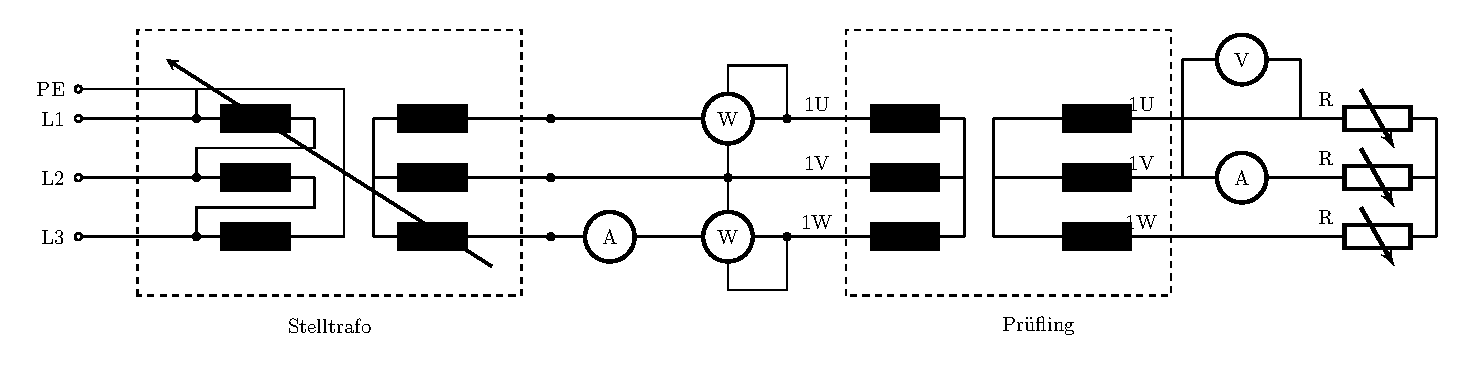
\includegraphics[width=0.95\textwidth]{fig/ohm_mess.pdf}
    \caption{Messschaltung Ohmische Belastung }
    \label{fig:my_label}
\end{figure}
\begin{figure}[H]
    \centering
	\begin{subfigure}{6cm}
	  \centering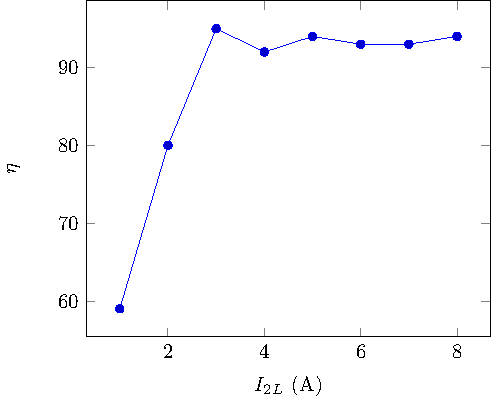
\includegraphics[width=6cm]{fig/r_eta.pdf}
	\end{subfigure}
	\begin{subfigure}{6cm}
	  \centering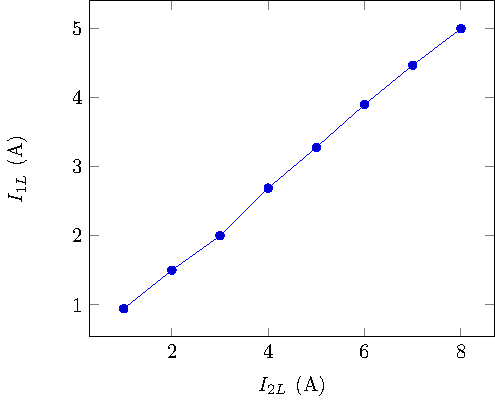
\includegraphics[width=6cm]{fig/r_i1i2.pdf}
	\end{subfigure}

	\begin{subfigure}{6cm}
	  \centering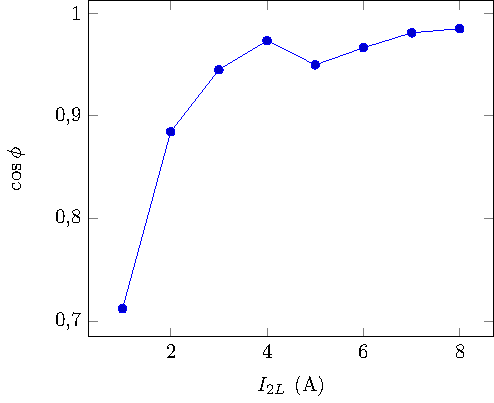
\includegraphics[width=6cm]{fig/r_pf.pdf}
	\end{subfigure}
	\begin{subfigure}{6cm}
	  \centering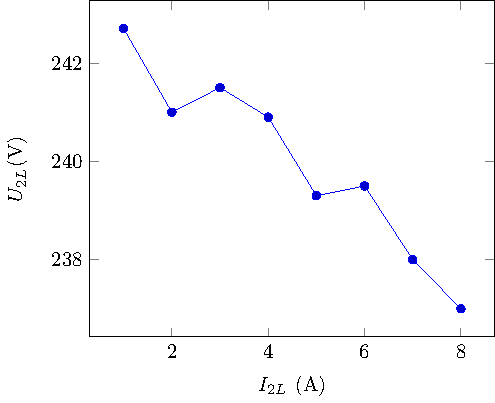
\includegraphics[width=6cm]{fig/r_u2i2.pdf}
	\end{subfigure}
	\caption{SOME CAPTION!}
  \end{figure}

